\section{Функционал шаардлагууд}
\begin{itemize}
      \item \textbf{ФШ 100:} Систем нь цахим баримт бичгүүд болон лицензийн талаарх мэдээллийг найдвартай байдлыг хадгалахын тулд Ethereum блокчэйн-тэй харилцах ёстой.
      \item \textbf{ФШ 200:} Цахим баримт бичгүүд эзэмших, лиценз олгох асуудлыг зохицуулахын тулд ухаалаг гэрээг блокчейн дээр байршуулж, удирдах ёстой.
      \item \textbf{ФШ 300:} Систем нь цахим баримт бичгүүдийг байршуулах, лиценз авахын тулд  хэрэглэгчийн крипто хэтэвчтэй холбогдсон байх ёстой.
      \item \textbf{ФШ 400:} Систем нь хэрэглэгчид вэб аппликейшны интерфейсээр дамжуулан PDF файлуудыг байршуулах боломжтой байх ёстой.
      \item \textbf{ФШ 500:} Систем нь цахим баримт бичгүүдийг байршуулахдаа баримт бичгийн мэдээллийг бүртгэх ёстой.
      \item \textbf{ФШ 600:} Систем нь цахим баримт бичиг байршуулах үед систем нь файлын хэшийг тооцоолж, хадгалалтыг үргэлжлүүлэхийн өмнө давхардсан эсэхийг шалгах ёстой.
      \item \textbf{ФШ 700:} Систем нь цахим баримт бичиг байршуулах үед систем нь файлын хэшийг тооцоолж, хадгалалтыг үргэлжлүүлэхийн өмнө давхардсан эсэхийг шалгах ёстой.
      \item \textbf{ФШ 800:} Хэрэглэгчид байршуулсан цахим баримт бичгүүдийн лицензийг авах боломжтой байх ёстой.
      \item \textbf{ФШ 900:} Цахим баримт бичгийн лиценз авахад лицензед өвөрмөц дугаар олгож, блокчейн дээр хадгалах ёстой.
      \item \textbf{ФШ 1000:} Систем нь хэрэглэгчид лиценз авсны дараа лицензийн дугаар, файлын мэдээлэл зэрэг лицензийнхээ дэлгэрэнгүй мэдээллийг агуулсан цахим гэрчилгээ авах ёстой.
      \item \textbf{ФШ 1100:} Хэрэглэгчид cистем дээр байрлуулсан цахим баримт бичгүүдийн дэлгэрэнгүй мэдээллийг үзэх боломжтой байх ёстой.
\end{itemize}

\section{Функционал бус шаардлагууд}
\begin{itemize}
   \item \textbf{ФБШ 100:} Блокчейн технологи нь өгөгдлийн бүрэн бүтэн байдлыг хангаж, лицензийн мэдээллийг зөвшөөрөлгүй өөрчлөхөөс сэргийлнэ.
      \item \textbf{ФБШ 200:} Систем нь гүйцэтгэлийн бууралтгүйгээр олон тооны хэрэглэгчид болон лицензүүдийг зохицуулах чадвартай байх ёстой.
      \item \textbf{ФБШ 300:} Ухаалаг гэрээ нь модульчлагдсан байх ёстой бөгөөд шинэчлэгдэхэд хялбар байх ёстой.
      \item \textbf{ФБШ 400:} Систем нь хүлээн зөвшөөрөгдсөн тодорхой хугацааны дотор баталгаажуулах хүсэлтийг хурдан боловсруулах чадвартай байх ёстой.
      \item \textbf{ФБШ 500:} Систем нь янз бүрийн техникийн чадвартай хэрэглэгчдэд үүнийг үр дүнтэй ашиглах боломжийг олгодог хэрэглэгчдэд ээлтэй интерфэйстэй байх ёстой.
      \item \textbf{ФБШ 500:} Систем нь янз бүрийн үйлдлийн систем, хөтөч, төхөөрөмжтэй нийцтэй байх ёстой.
      \item \textbf{ФБШ 600:} Систем нь лиценз олгох, дижитал гүйлгээ, блокчэйн технологитой холбоотой аливаа зохицуулалтын шаардлагад нийцэж байх ёстой.
      \item \textbf{ФБШ 700:} Энэ систем нь гамшгийн үед өгөгдөл алдагдахгүй байхын тулд найдвартай нөөцлөх, сэргээх механизмтай байх ёстой.
\end{itemize}

\newpage
\section{Use case диаграм}
\begin{figure}[h]
	\centering
	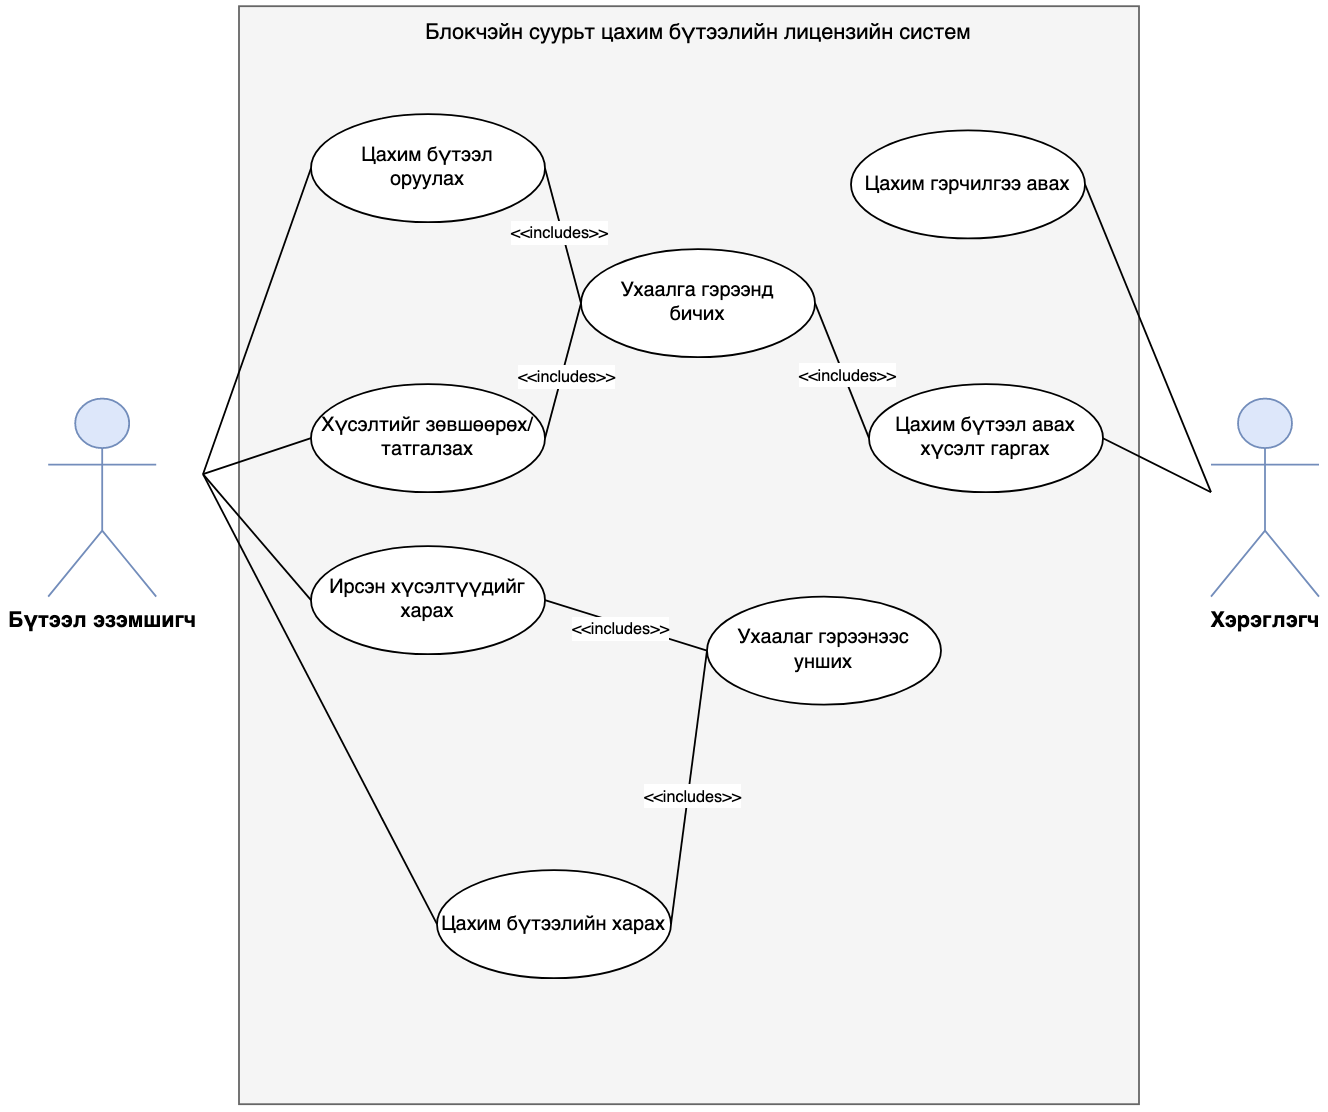
\includegraphics[scale=0.4]{src/images/usecase.png}
	\caption{Use-case диаграм}
\end{figure}


\section{Архитектур}
Энэхүү төслийг ажиллахад илүү хямд зардалтай хүртээмжтэй, ачаалал даах чадварыг
нэмэх зорилгоор серверлесс Архитектур сонгосон юм. Фронт-энд хэсэг нь NextJS-н ашигласан тул Сервер талын рендер хийж байгаа ба хэрэглэгчийн оруулсан цахим баримт бичиг болон лицензийн мэдээллийг Этереум блокчэйн сүлжээнд бичих болон унших үйлдлийг хийх юм. Мөн хэрэглэгчийн оруулсан цахим баримт бичгийг IPFS сүлжээнд хадгална.

\begin{figure}[h]
	\centering
	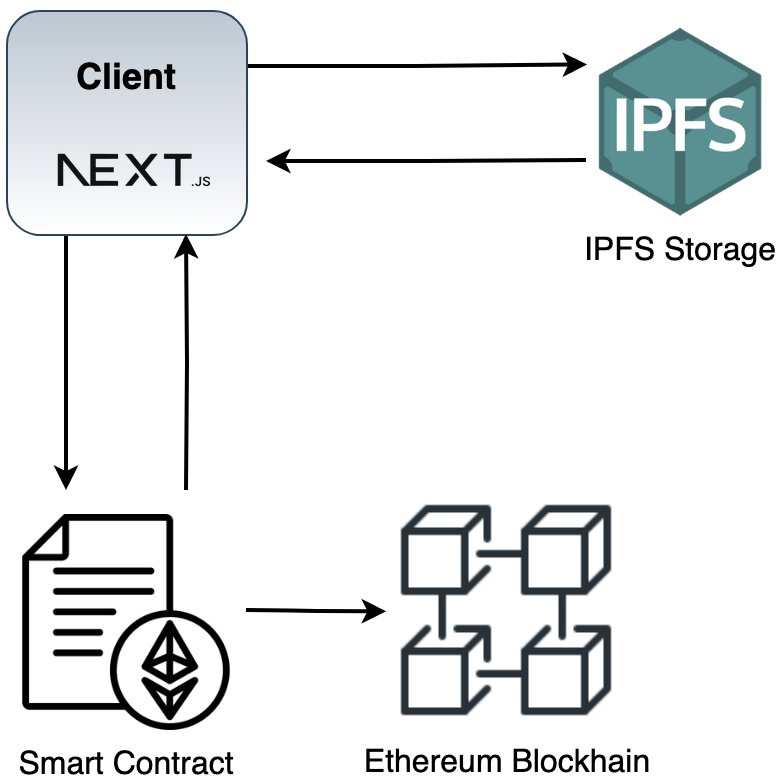
\includegraphics[scale=0.4]{src/images/architecture.png}
	\caption{Архитектурын зураг}
\end{figure}
